\epigraph{I was born not knowing and have only had a little time to change that}
{\textit{Richard P. Feynman}}

\section{The Mindset Shift}

At school, I was used to understanding things quickly. 

If I didn't understand something in class, I usually would by the end of the lesson. And if I didn't, I could go home, do a few questions, and it would click. There was a clear structure, you learned a method, applied it, and got better. 

University maths felt different almost immediately. 

Having worked at a department open days, one of the most common questions I get asked is `What's the jump actually like? Is it just harder? Is it just more content?' 

My honest answer has been and still is: it's just different. 

One of the most common issues that students face, and this is more than just my personal experience, is that they no longer understand things straight away. This was something which I recall being addressed on numerous university open days when I was still in school, but I didn't truly understood what that meant until I got to university. 

Often at school, not understanding usually meant you needed more practice. However at university, not understanding often meant to me that I needed more time, or more reflection, or just a shift in how I was used to thinking. This is especially true if you are used to being the `the maths person', and used to being the one who got it first. The point I want to convey is that the jump isn't just academic, it's also psychological. 

\section{Why Maths is Different}

In many subjects or courses, you can revise by memorising key ideas, reading around the topic or absorbing information repeatedly until it sticks. 

Mathematics doesn't work like that. You can't (always) memorise your way into deep understanding or skim a proof and expect it to feel natural. You can't treat definitions and just some vocabulary words and hope they'll make sense. 

One of the best things I like about university maths is that it shifts the focus from `doing' to `justifying'. You go from merely applying formulas to understanding why those formulas exist in the firs place, and from being shown the path to a theorem to learning how to build the path yourself. 

You might be used to mastering a particular technique or a method from school, and those skills continue to be useful when you transition to university, but more often than not, you find yourself exploring structure. And exploration is slower, but also more rewarding. 
 

\section{Redefining Understanding}

The underlying issue in my experience is often to do with expectation students have from themselves rather than their level of intelligence. 

Mathematics is a conceptually difficult subject to grasp. If you approach each lecture or assignment with the mindset that you're expected to understand everything, or feeling confused means you're not good enough, the delay or lack of those things can feel like failure. 

Having such expectations from yourself are completely understandable and they might've worked well before, but you might find that they don't work in the same way now. Maths is build on layers. You might understand the notation before the idea, or follow a proof before you really see why it's necessary.

If you ever feel confused or find yourself struggling, rest assured, you're not alone. It's incredibly common, normal, and all part of the process. 

Now for the challenging part, you have to let go of the need to understand everything immediately. This doesn't mean lowering standards, but adjusting expectations as discussed in the section above. 

Understanding at the level at which university maths progresses takes time. It requires sitting with new ideas and concepts you might've never seen before. Trying things that don't work, and being okay with not being the fastest or the brightest in the room. It's less about speed and more about structure. 

The jump isn't just from `easy' to `hard'. I think it's more from procedural to conceptional, from the methods you might be familiar with, to the mindset shift you might have to make. And once you accept that, the confusion will hopefully start to feel less threatening. 


\begin{figure}
    \centering
    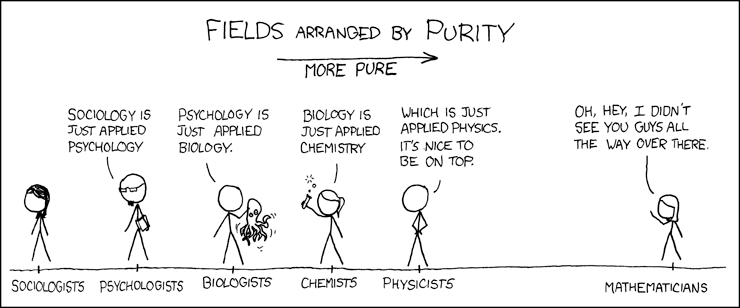
\includegraphics[width=0.5\linewidth]{xkcd/purity.png}
    \caption{\textbf{\href{https://xkcd.com/435/}{Purity}}}
\end{figure}